\section{Overview of Mining GCMP in Parallel}
\label{sec:system_overview}
We adapt the MapReduce paradigm for designing
a parallel solution of mining GCMP. MapReduce was proposed by Dean et. cl.~\cite{}
and has become a mature parallel platform for large-scaled data processing. 
Current open source MapReduce systems provide handy programming APIs with fault tolerances
in backends. Such systems 
include Apache Hadoop, Apache Shark and Apache Spark to name a few.

In simple words, there are two types of cluster nodes in MapReduce, namely the 
\emph{mapper}s and the \emph{reducer}s. The execution of a MapReduce task consists of
three stages: First, input data
are partitioned and read by a \emph{map} function on each mapper. Then, mappers
emit key-value pairs which are \emph{shuffle}d over the network to reducers. Finally,
reducers process received data using a \emph{reduce} function then write the
outputs.
Since the \emph{shuffle} stage needs to transfer data over network, 
an important attention to pay during designing MapReduce algorithms is 
to minimize the shuffle amounts and shuffle counts. 

Our GCMP mining workflow follows the MapReduce style which consists of five stages
as illustrated in the Figures~\ref{fig:overview} (a)-(e).
As shown, in stage (a), trajectory data 
are read from various sources and partitioned based on objects timestamps, where objects
of the same timestamps form a snapshots. After partitioning, snapshots are send to workers
prior to stage (b). In stage (b), objects belonging to the same snapshots are clustered
based on the user supplied clustering method. Then those clusters are shuffled to 
workers prior to stage (c). In stage (c), each worker collects the clusters sent to its partition
and discover the GCMP from these local clusters. A post-check is required to remove
duplicate patterns. In stage (d), patterns discovered in previous stages are write to output.


\begin{figure} [t]
\center
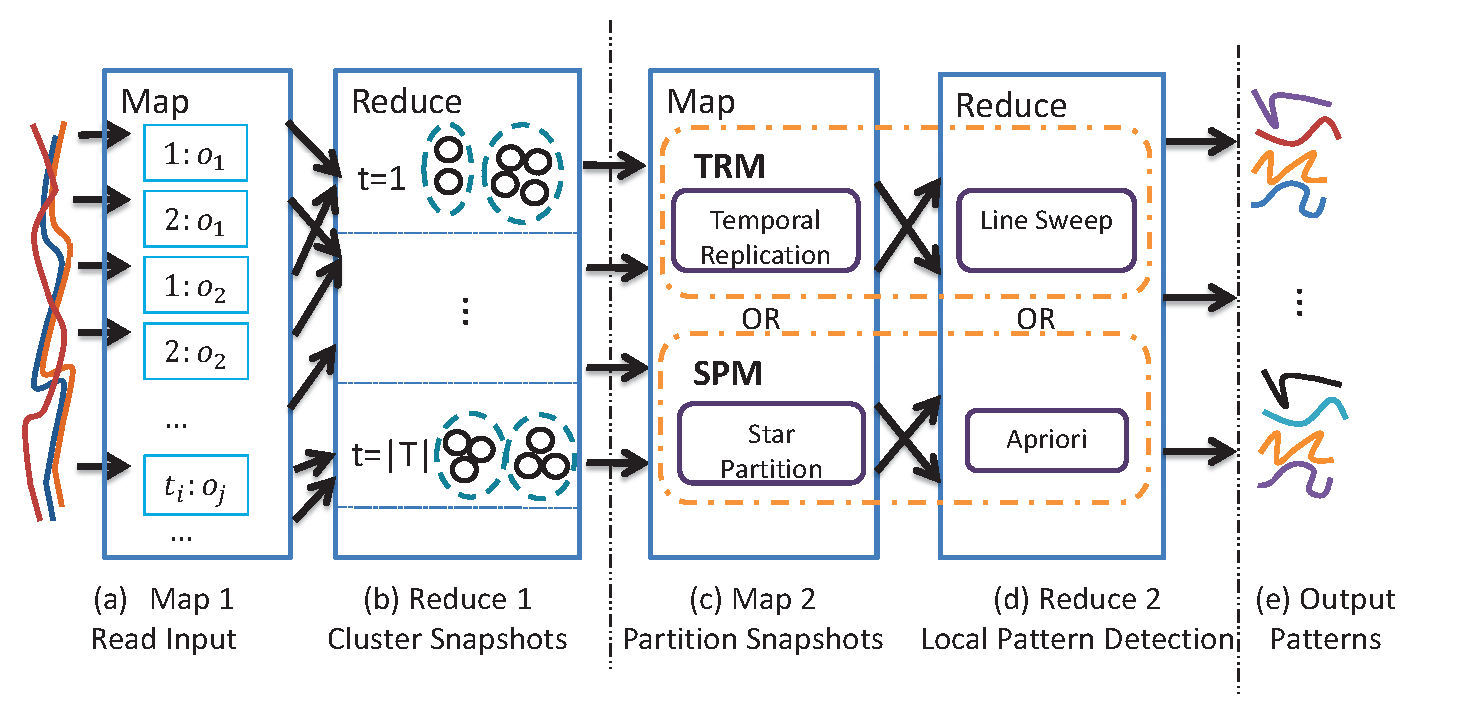
\includegraphics[width=0.5\textwidth]{system_layout.eps}
\caption{System Flow of Mining GCMP}
\label{fig:overview}
\end{figure}


The first two stages of our solution could be straightforward. 
However, it is challenging to design the partition and mining methods
to in stage (c) and (d). Intuitively, A reasonable partition strategy 
needs to meet the following requirements: first, the result partitions need
to preserve enough information so that real patterns can be discovered
in stage (d). Second, the result partitions need to ensure that
the patterns that discovered in stage (d) are real patterns so that
no further validation is required after stage (d). We formalize the two 
properties using \emph{completeness} and \emph{soundness} as follows:

\begin{definition}[Completeness and Soundness]
Let a partition method $\mathbb{P}$ partitions original trajectories $Tr$ into multiple parts, $Par_1,...,Par_m$. $\mathbb{P}$ is complete if for every pattern $P$ that is valid in $Tr$, $\exists Par_i$ such that $P$ is valid in $Par_i$. $\mathbb{P}$ is sound if for all patterns $P$ that is valid in any $Par_i$, it is also valid in $TR$.
\end{definition}
The completeness ensures that no real patterns are missed out. The soundness ensures that no false patterns are reported. If a partition method is both sound and complete, we are then able to mining patterns in each resulted partition in parallel in stage (d). 

Apparently replicating entire data set to each partition meets the \emph{soundness} and \emph{completeness}, however, it burdens the network shuffle and GCMP mining. Our objective is thus to design a complete and sound partition method that
minimize the network shuffles.

%Depends on the pattern mining strategy, the size of shuffle and replication may differ. We show that if the pattern mining strategy is not selected carefully, the second stage will suffer from large data replication and shuffling.


%
%In particular, we need
%the number of partitions to be reasonably large in order to achieve
%good parallelism in stage (d). Meanwhile, we need to ensure a partition 
%of snapshots containing enough information so that patterns discovered 
%in stage (d) are complete.  Furthermore, we have to ensure that the
%patterns that discovered in stage (d) are real patterns.

%However, there are two conflicting requirements that restrain us from 
%designing a simple and effective solution. 
%On one hand, we need to partition snapshots in stage (c) as many as possible 
%so that good parallelism could be achieved in stage (d). 
%On the other hand, in stage (d), 
%we require each partition containing enough information in order to discover
%proper GCMP patterns. This prevents us from arbitrarily partition snapshots in
%stage (d). To design a working algorithm, find the minimum size of partition is
%crucial. In the following section, we first design a naive approach that
%partitions snapshots by allowing overlapping among partitions. Such a partition strategy
%although has overhead in shuffling, it corrects find GCMPs in parallel in stage (d).
%In order to discover all patterns, we require a partitioning method to be \emph{complete} and \emph{Sound}. 

%\section{Temporal Replication and Mining}
%
%
%%It is notable that some patterns 
%%may be very long in duration (e.g., when discovering \emph{swarm}) or some patterns 
%%may contain a large set of objects (e.g., when discover \emph{group} patterns with small $L$).
%%Therefore, we require the size of partition to be large enough. Reaching the
%%balance between the two requirement is crucial. In the following sections, we will
%%describe a naive partition scheme which meets the two requirements.
%
%%Our parallel solution incurs two rounds of shuffles. The first round of shuffle happens in step (a). This
%%is because that the trajectories stored in HDFS needs to be regrouped to form snapshots. 
%%The second round of shuffle occurs in step(d). This is because that 
%% the clusters need to be regrouped so that subsequent pattern detection can be performed.
%% Despite the simpleness of our parallel solution, it is actually nontrivial to work out a scalable solution.
%% The major challenge lies in the step (d) and (e). 
%
%
%%\section{Preliminary on Apache Spark}
%%\label{sec:system_overview}
%%Apache Spark is an open sourced modern parallel processing platform
%%based on Resilient-Distributed-Dataset (RDD). Each RDD is able to take an action (including Map, Reduce, GroupByKey etc.) and then transforms to a new RDD. Algorithms in Spark is implemented by supplying various actions to an input RDD. Each RDD in Spark has a pre-defined and fixed number of partitions, where each partition forms a task assigned to an executor.
%%
%%Compared to MapReduce, Spark 
%%utilizes distributed memory to cache the programming data modeled as RDDs, which brings computational benefits~\cite{shi2015clash}. In order to fully utilize the memory, Spark creates one thread for each task and then multiple tasks belonging to the same JVM share the available memory.
%Due to threading, there is a paradigm shift from MapReduce to Spark. In MapReduce, the cost of starting a task is expensive, as each task in MapReduce requires a dedicated JVM process. While in Spark, the cost of starting a task is negligible since each task is done by a thread.  Therefore in Spark, we may create many more parallel tasks than in MapReduce before reaching to the system limitation.


%\section{Mining Generalized Co-moving Pattern}
%\label{sec:solution}
%There are two stages in mining GCMP. The first stage is to cluster objects in each snapshots. Then the seconds stage is to mine patterns from clusters in parallel. The overview of the parallel approach is 
%shown in Figure~\ref{fig:overview}. As shown, trajectory data is initially stored in HDFS. The first stage is to 
%read trajectories and cluster objects in the same snapshots. Since the objects at each snapshots are independent, this stage can be easily performed in parallel. The first stage involves network IO. Afterwards, the clusters in each snapshots are shuffled and replicated to make various partitions.


\section{Temporal Replication and Mining}
The straightforward strategy of parallelizing the second stage is to vertically partition the trajectories based on snapshots. 
A simple but effective method
is to group neighborhood snapshots into a partition, such that every possible pattern can be mined within some of the partitions. In order to achieve the \emph{completeness},
some of the snapshots need to be replicated on multiple executors.
We call this method the \emph{Temporal Replication and Mining} approach. 
The algorithm is presented as in Algorithm~\ref{algo:trm_overview}.

\begin{algorithm}
\caption{Temporal Replication and Mining}
\label{algo:trm_overview}
\begin{algorithmic}
\Require list of $\langle t, S_t \rangle$ pairs
\State {Map Phase}
\ForAll{$\langle t, S_t \rangle$}
	\ForAll{$i \in 1...(K-1)*G+K$}
		\State emit a $\langle t-i, S_t \rangle$ pair
	\EndFor 
\EndFor
\State {Shuffle Phase}
\ForAll{$\langle t, S \rangle$ pair} 
\State group-by $t$, emit a $\langle t, Par_t\rangle$,
\State  where $Par_t = \{S_t, S_{t+1}, .. S_{t+(K-1)*G+K}\} $
\EndFor
\State {Reduce Phase}
\ForAll{$\langle t,Par_t \rangle$}
\State minePattern($Par_t$)
\EndFor

\end{algorithmic}
\end{algorithm}


\subsubsection{Temporal Replication Partition}
In order to reduce the shuffling cost, the data to be replicated should be
kept to a minimum. However, as suggested in the following theorem, the minimum replication of a snapshot is not small:

\begin{theorem}[Soundness and Completeness of Replication]
\label{thm:replication_partition}
For each snapshot $S_t$, a partition $Par_t = \{S_t, ...,S_{t+(\lfloor \frac{K}{L}-1\rfloor *G+K)}\}$ 
is created. Such a partition method is sound and complete.
\end{theorem}
\begin{proof}
The soundness of partition is trivially true by definition.
Given a valid pattern $P$, let $T' \subseteq P.T$ be a subsequence of $P.T$ which conforms to $K,L,G$. Note that there could be many qualified $T'$ of $T$. Then, 
let the $i^{th}$ local-consecutive part of $T'$ be $l_i$ and let the $i^{th}$ gap of $T'$ be $g_i$. Then, the size of $T'$ can be written as $\Sigma_i (l_i + g_i)$. Since $T'$ conforms to $K,L,G$, then $\Sigma_i (l_i) \geq K$, and $K \geq l_i \geq L$, $g_i \leq G$. Therefore, among all possible $T'$s, the minimum size is $\lfloor \frac{K}{L}-1\rfloor *G+K$. Thus ensuring each $Par_t$ to be of that size would capture one of the $T'$s, therefore the pattern $P$ is valid in $Par_t$. This proves the completeness of the partitioning method.
\end{proof}

Utilizing Theorem~\ref{thm:replication_partition}, we create, for each snapshot $S_t$, 
a partition containing its next $\lfloor \frac{K}{L}-1\rfloor *G+K$ snapshots. Each partition is then
sent to the executors as a task. Since any global pattern must exists in one of the partitions, we can mine the patterns from each partitions independently, without loss of patterns.

\subsubsection{Temporal Replication Mining}
After replication, each task in Spark will process an partition $Par_i$. The next
step is to mine the GCMPs from $Par_i$. We notice that, for each 
partition, we only need to find the patterns that
are contained in the first snapshots. Therefore we design a line-sweep method for mining 
such patterns, which is the variant of the Coherent-Moving-Clustering method in~\cite{jeung2008convoy}.

The Temporal Replication and Mining approach though achieves parallelism from independent
partitions, it requires to replicate the data multiple times. 
Specifically, each snapshots are copied $(K-1)*G+K$ times. In swarm
case, $G$ is as large as $|\mathbb{T}|$. In such a case, it is equivalent to replicate the entire dataset 
to each executor, which is clearly inefficient.


\subsection{Star Partition and Mining}
To develop a method that achieves parallelism under any pattern parameters, 
we propose the \emph{Star Partition and Mining} (SPM) method. In SPM,
we design a novel object-based partition method named star partition. A start partition partitions trajectories in the object domain rather than temporal domain. After partitioning, we design the \emph{Apriori}-like 
method to mine the patterns out of each partition independently. 
The overview of the star partition and mining is as in Algorithm~\ref{algo:spm_overview}.

\begin{algorithm}
\caption{Star Partition and Mining}
\label{algo:spm_overview}
\begin{algorithmic}
\Require list of $\langle t, S_t \rangle$ pairs
\State {Map phase}
\ForAll{$C \in S_t$}
	\ForAll {$(o_1 ,o_2) \in C \times C$}
		\State emit a $\langle o_1, o_2, \{t\}\rangle$ triplet
	\EndFor
\EndFor

\State {Shuffle phase}
\ForAll{$\langle o_1, o_2, \{t\}\rangle$ triplets} 
	\State group-by $o_1$, emit $\langle o_1, Sr_{o_1} \rangle$ 
	\State group-by $o_2$, emit $\langle o_2, Sr_{o_2} \rangle$
\EndFor

\State {Reduce phase}
\ForAll{$\langle o, Sr_{o} \rangle$}
\State Apriori($Sr_o$)
\EndFor

\end{algorithmic}
\end{algorithm}

\subsubsection{Star Partition}
The purpose of star partition is to find the group of objects that 
could potentially form a pattern. In order to achieve parallelism, 
we group, for each object $o$, all other objects that connect to $o$ in some snapshots. By so doing, the patterns containing $o$ can be discovered within each groups. 
Technically, we create a connection graph to represent the
connectivity among objects. A connection graph is an undirected graph $G=(V:E)$, where 
each $v \in V$ represents an object. An edge $e(s,t)= ET$ 
contains all the timestamps where $s,t$ are in the same cluster,
i.e., $\forall t \in ET, C_t(s) = C_t(t)$. 
Given a vertex $s$, the star of $s$, $Sr_s$ is the set of incidental edges of $s$ in $G$. An example of star partition is shown in Figure~\ref{fig:star_partition}.

\begin{figure}[h]
\centering
\includegraphics[width=0.5\textwidth]{star_partition.jpg}
\caption{Example of Star Partition}
\label{fig:star_partition}
\end{figure}


In star partition, trajectories are partitioned based on objects and their stars. Then
each partition is send to an executor as a task. 
Indeed, a star $Sr_s$ can be viewed as a subset of original trajectories. This is done by treating each vertex in $Sr_s$ as an object. For $s$, the time sequence is the union of all edges in $Sr_s$. For vertex $v \neq s$, the time sequence is the edge $(s,v)$.
Then, we state the completeness of star-partition as in the following theorem:
\begin{theorem}[Soundness and Completeness of Star Partition]
Star partition is sound and complete.
\end{theorem}

\begin{proof}
For the soundness,
if $P$ is a valid pattern in $Sr_s$, then for every object $v\neq s, v \in P.O$, and for every timestamp $t\in P.T$, $C_t(v) = C_t(s)$. This means, for every snapshot $t$, all object in $P.O$ belongs to the same cluster. Thus, $P$ is a valid pattern in original trajectories.

For the completeness,
if $P$ is a valid pattern in original trajectories, for an arbitrary object $s \in P.O$, it follows $P.O \equiv S_r$. Since for any time $t$, $C_s(t) = C_v(t) \forall v \in P.O$, every time in $P.T$ appears in edges in $Sr_s$, thus $P$ is valid pattern in $Sr_s$.
\end{proof}

Based on the above theorem, each star can be processed independently by executors, which avoids the inter-executor communication during the mining phase. It is notable that, the 
replication of data is $O(|\mathbb{O}|^2|\mathbb{T}|)$, which is free from the parameters of patterns.
In later sections, we will describe optimization techniques to reduce the replications.

\subsubsection{Apriori Mining}
For each task, in the mining phase, we need to find the patterns that conform to the parameters. To systematically discover the patterns, we design the \emph{Apriori Mining} method which
is similar to frequent item mining. During the algorithm, we call a candidate pattern $R$-pattern if the size of its object set is $|R|$. 
Our algorithm runs in iterations. During each iteration $R$, we try to generate all $(R+1)$-patterns. In iteration $1$, the $2$-pattern is the edges in $Sr_s$. In particular,
for each $e(s,v)=ET$, pattern $p=(\{s,v\}, ET)$ is formed. During each iteration, 
we generate $(R+1)$-cluster patterns by joining $R$-cluster patterns with $2$-cluster patterns. Specifically,
the join between $p_1=(O_1, T_1)$ and $p_2=(O_2, T_2)$ would generate a new pattern $p_3=(O_1 \cup O_2, T_1 \cap T_2)$. Notice that in $Sr_s$, each $R$-pattern consists of the object $s$, thus the join will grow a $R$-cluster at most to a $(R+1)$-cluster.
Our mining algorithm stops where no further patterns are generated. The algorithm is illustrated as in Algorithm~\ref{algo:apriori_mining}.

\begin{algorithm}
\caption{Apriori Mining}
\label{algo:apriori_mining}
\begin{algorithmic}
\Require{$Sr_s$}
\State { Lv $\gets \{\}$}
\State { Ground $\gets \{\}$}
\ForAll{$e(s,t) = T \in Sr_s$}
\State Ground.add($\langle \{s,t\}, T \rangle$);
\State Lv $\gets$ Ground;
\EndFor
\While{true}
	\If{Lv is not empty} 
		\State{LvCand $\gets \{\}$ }
		\ForAll{$cand_v \in Lv$}
			\ForAll{$cand \in $Ground}
				\State $p \gets cand_v$ join $cand$
				\If{$p.T$ is partly valid} 
					\State LvCand.add($p$)
				\EndIf
			\EndFor
		\EndFor
		\State {Lv $\gets$ LvCand}
	\Else
		\State{break}
	\EndIf
\EndWhile
\end{algorithmic}
\end{algorithm}

Algorithm~\ref{algo:apriori_mining} takes exponential complexity to mine GCMP. There
are two major factors dragging the performance. First, the size of $Sr_s$ affects
the initial size of $2$-patterns. Second, the candidates generated in each level affects the join performance. In later
sections, we exploit the property of GCMP to reduce the two factors.